\documentclass[11pt]{article}
\usepackage[margin=2cm]{geometry}
\usepackage{graphicx}
\usepackage{amsmath,amssymb}
\setlength{\parindent}{0pt}\setlength{\parskip}{5pt}
\graphicspath{{./}}
\begin{document}
\begin{center}{\Large\bfseries Base Driver --- Figure Notes for the Defense}\\[2pt]
6 deterministic episodes, gate 0.6~m, 6/6 success ($=100\%$); mean 56.7 decisions to reach (median 48.5), mean min distance 0.5286~m. Date 2026-09-24.\end{center}
\vspace{4pt}
\section*{Figure 1 --- Convergence to the target}
\begin{center}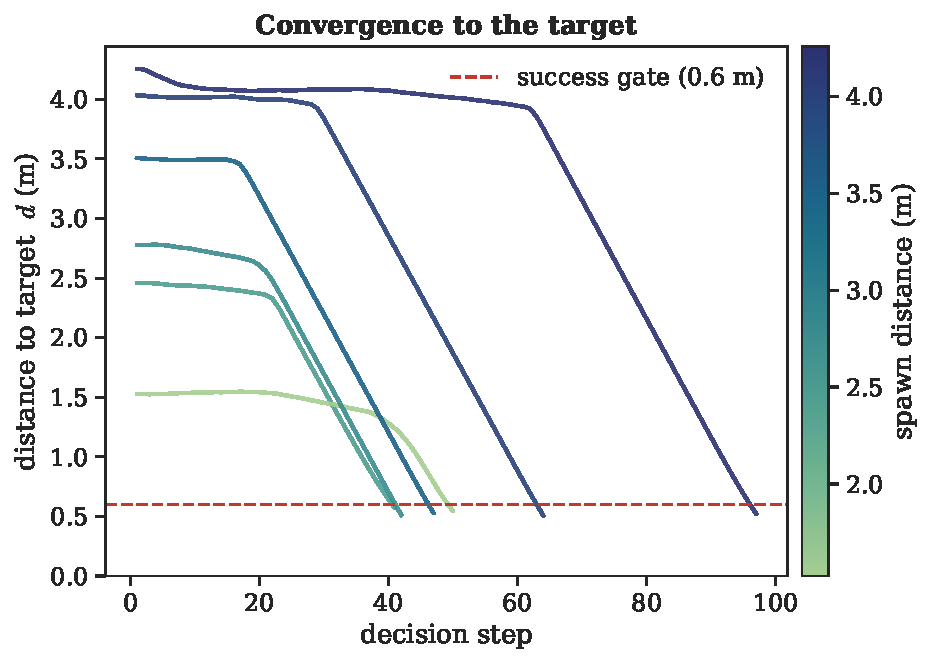
\includegraphics[width=0.80\textwidth]{base_eval_convergence.pdf}\end{center}
\textbf{What it shows.} For each of the 6 evaluation episodes, the distance from the base to the target versus decision step. Colour encodes how far the target spawned (dark = far); the red dashed line is the 0.6~m success gate.

\textbf{How to read it.} Every curve crosses below the gate: the base reaches the target in all 6 episodes (6/6). Each curve is roughly flat at first (the base turns in place, so distance barely changes) then descends almost linearly (it drives at near-constant speed).

\textbf{Say this.} ``The policy succeeds on 100\% of episodes. The flat-then-linear shape is a clean turn-then-drive strategy --- no curved, wasteful paths.''

\textbf{If asked.} \emph{Why the initial plateau?} --- The base first reduces its heading error (see the alignment figure) before translating, so the distance stays roughly constant during the turn.
\clearpage
\section*{Figure 2 --- Target approach in the robot frame}
\begin{center}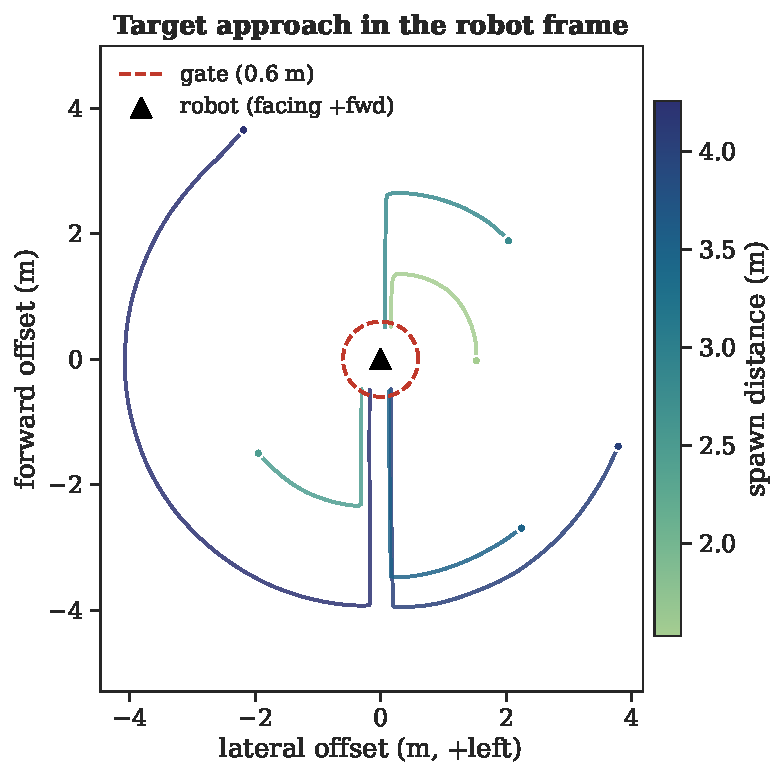
\includegraphics[width=0.80\textwidth]{base_eval_approach.pdf}\end{center}
\textbf{What it shows.} The target's position expressed in the base's own frame over each episode. The base sits at the origin (triangle) facing $+$forward; the red circle is the 0.6~m gate; dots mark the target at spawn.

\textbf{How to read it.} Targets start in every direction --- ahead (positive forward offset), behind (negative), left or right --- and every trace funnels into the gate circle. The wide arcs are episodes where the target was behind: as the base rotates to face it, the target sweeps across the frame.

\textbf{Say this.} ``In the robot's own reference frame, targets from any direction --- including directly behind --- are brought into the success gate. The FLU policy covers the full 360$^\circ$.''

\textbf{If asked.} \emph{Why do paths curve instead of going straight?} --- This plot is in the \emph{moving} robot frame; the target appears to arc because the robot is rotating. In the world frame the base path is turn-then-straight.
\clearpage
\section*{Figure 3 --- Effort scales with spawn distance}
\begin{center}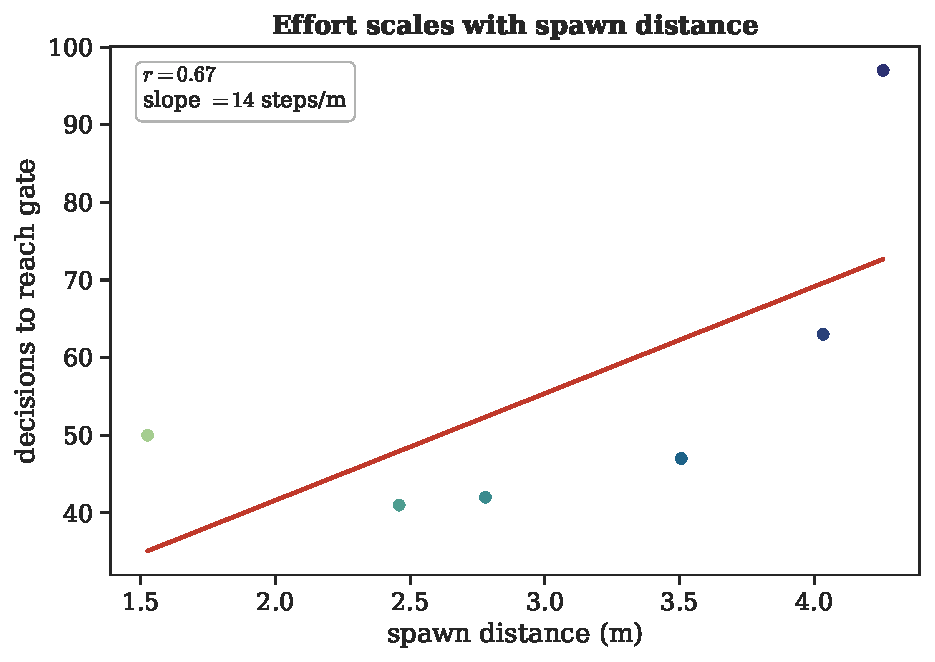
\includegraphics[width=0.80\textwidth]{base_eval_scaling.pdf}\end{center}
\textbf{What it shows.} Decisions needed to reach the gate versus spawn distance, one point per episode (spawns 1.5--4.3~m), with a least-squares line. Pearson $r=0.67$, slope $\approx 13.8$ steps/m.

\textbf{How to read it.} Points trend upward --- farther targets take more decisions --- and the positive slope quantifies it: about 13.8 decision steps per additional metre.

\textbf{Say this.} ``Time-to-goal grows roughly linearly with distance, exactly what a constant-speed driver should do --- the policy adds no overhead for far targets.''

\textbf{If asked.} \emph{Is 6 episodes enough to claim linearity?} --- It is a qualitative trend on 6 deterministic episodes; I report it as indicative and would expand to more episodes for a tight regression estimate.
\clearpage
\section*{Figure 4 --- Alignment: heading error over time}
\begin{center}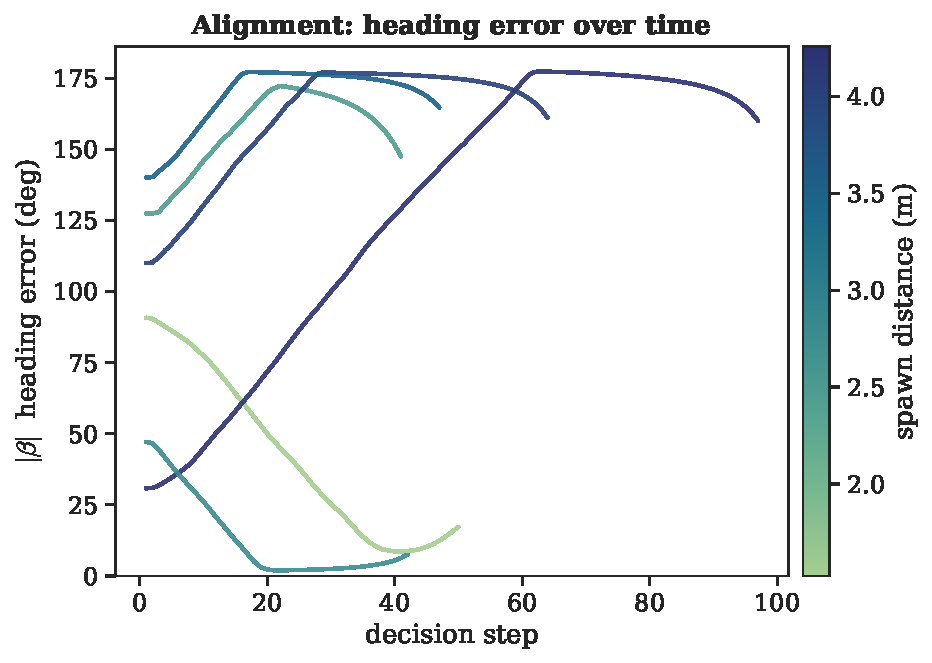
\includegraphics[width=0.80\textwidth]{base_eval_bearing.pdf}\end{center}
\textbf{What it shows.} The absolute heading error $|\beta|$ (angle between the base's facing and the target direction) versus decision step, per episode.

\textbf{How to read it.} All curves fall to near $0^\circ$ and stay there: the base aligns with the target and holds that alignment while driving in. Curves that first climb toward $180^\circ$ are targets that spawned behind --- the base swings around, briefly pointing away, before settling.

\textbf{Say this.} ``Heading error converges to near zero early and stays there --- the policy locks onto the target heading, then translates. That is why the distance curves are so straight.''

\textbf{If asked.} \emph{What is $\beta$ exactly?} --- The angle between the base's forward (or rear, whichever is nearer) axis and the direction to the target; $0^\circ$ means facing the target.
\clearpage
\section*{Figure 5 --- Overview (one-slide summary)}
\begin{center}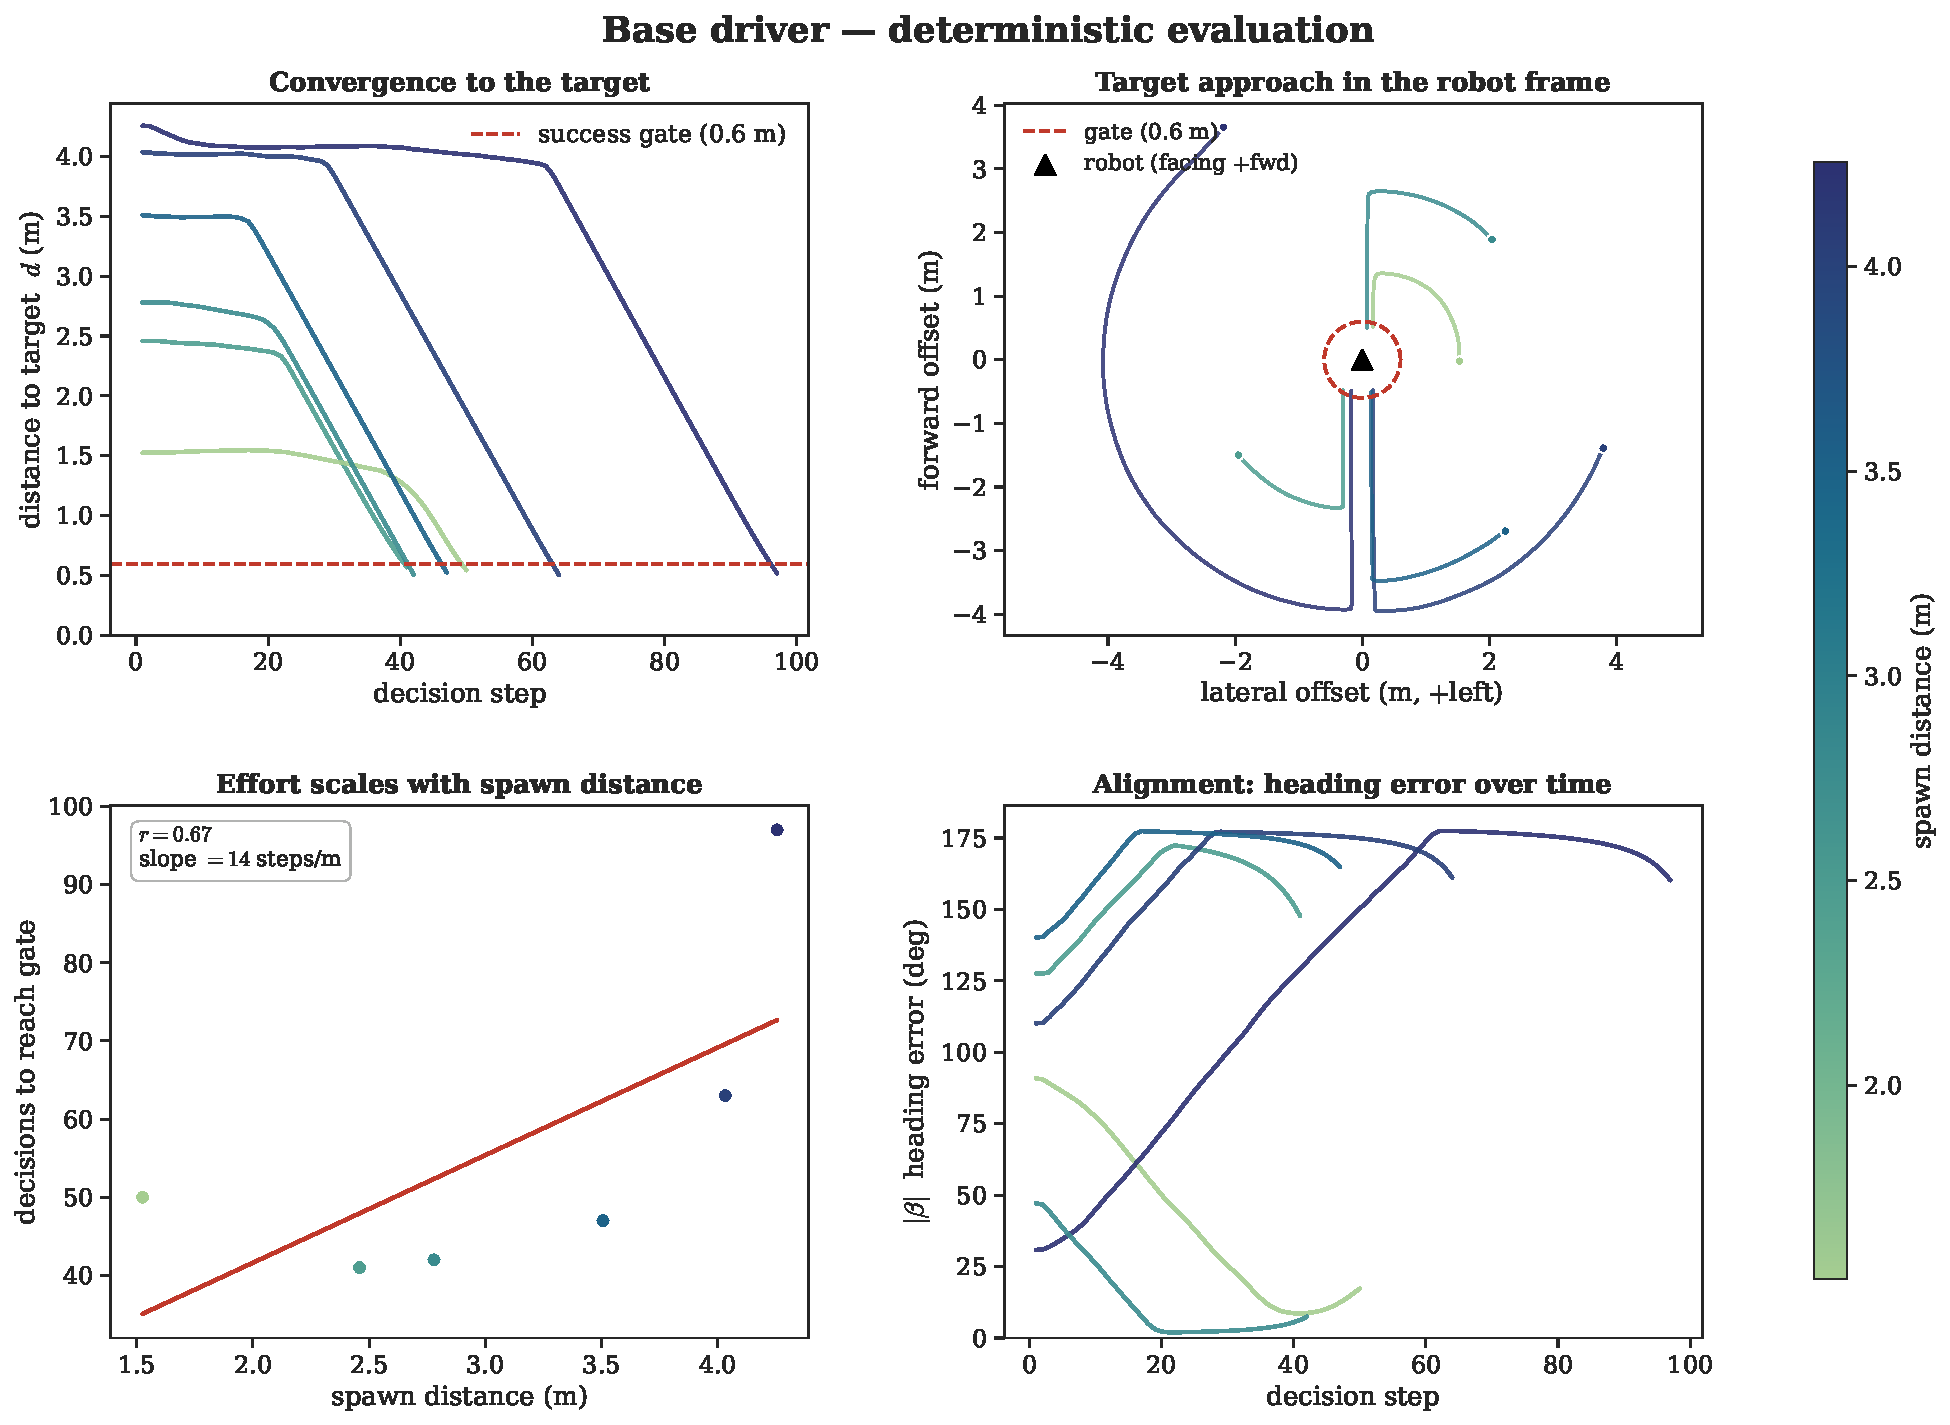
\includegraphics[width=0.80\textwidth]{base_eval_overview.pdf}\end{center}
\textbf{What it shows.} The four diagnostics on a single figure --- convergence, robot-frame approach, scaling, alignment.

\textbf{How to read it.} Use this as the summary slide; the four panels are described on the preceding pages.

\textbf{Say this.} ``The base driver reaches the target in 100\% of episodes (top-left), from any relative direction (top-right), in time that scales linearly with distance (bottom-left), by aligning first and driving second (bottom-right).''

\textbf{If asked.} \emph{One figure to remember?} --- This one: it captures success, generality, efficiency, and the turn-then-drive mechanism together.
\clearpage
\end{document}
